\chapter{Problem description}
\label{chap:problem}
% 1. As discussed in the introduction in order to facilitate the digital economy in the future an open, distributed reputation system is required. The reputation system will enable trustful relationships between strangers and will need to be at the core of the internet itself.  
% In the introduction we have made a case for our audacious ambition to design and create a layer 
% of reputation on top of the core infrastructure of the internet that enables application agnostic 
% trustful relationships between relative strangers. This requires a distributed, scalable reputation
% system. 

Our audacious long-term ambition is to create a global, distributed trust system. Such a trust system as a public, free and 
non-profit utility is a key element to enable next-generation online applications. In the 
previous chapter we have introduced trust research and the influential role trust plays in human 
society. The design complexities of such a system reach far beyond the scope of a single 
master thesis. In this chapter a specific problem will be defined that we identified as a crucial
challenge to solve in order to achieve the long-term goal.

\section{Model of trust and reputation}
Trust comes natural to people. Our intuition tells us from experience or some evidence who is 
trustworthy and who is not. This is not a failsafe process but it is the best we can do. If we try
to reason about this vague concept of trust or try to implement trust into an automated agent we
cannot use that intuition. Instead a model is needed which describes in explicit terms the 
concepts, and the relationships between them. This helps us to afterwards determine the components 
that are needed to create a fully capable trust system.

"A Computational Model of Trust and Reputation" by Mui et al.~\cite{mui2002computational} is an
important early work which provides a complete computational basis for those vague concepts. Mui
defines the concepts of trust and reputation in the context of an embedded social network. The 
network consists of a set of uniquely identifiable \textit{agents} that are able to interact with each other. 
Similar to the Prisoner's Dilemma agents either cooperate or defect in the \textit{encounter}. The incentive
for an agent to cooperate in encounters is the hope that the same agent or another agent will
return the favor and also cooperate in future encounters. Throughout their lifetime agents build a 
\textit{history} of encounters. The reputation of an agent is determined by that history. 

\begin{figure}[h!]
    \centering
    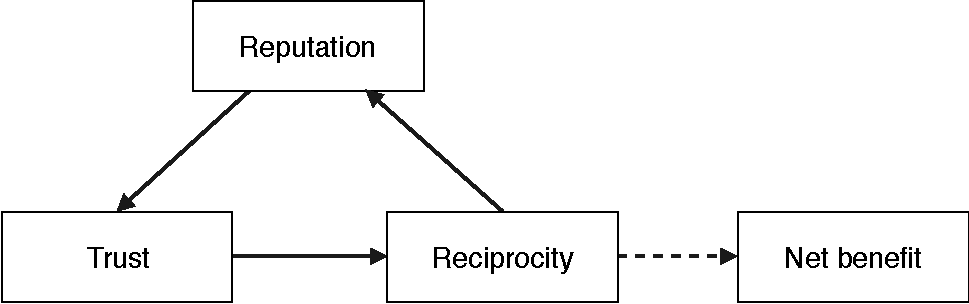
\includegraphics[width=\textwidth]{images/mui_figure.pdf}
    \caption{Self-reinforcing relation between trust, reputation and reciprocity. Source: Mui, 2002~\cite{mui2002computational}}
    \label{fig:mui}
\end{figure}

Trust and reputation can be calculated. For example, an estimator for the reputation
of an agent can be the number of encounters in which the agent reciprocated over the total number of 
encounters. Trust, is the probability that an agent will reciprocate in the next encounter given 
the agent's history. Mui et al.\ defines reputation as ``
perception that an agent creates through past actions about its intentions and norms''. A good 
reputation leads to trust from other agents. Their definition of trust as ``a subjective expectation
an agent has about another's future behavior based on the history of their encounters'' reflects
this. The more trust an agent has in another, the higher the probability for reciprocation in the following
encounter. This leads to another encounter of reciprocation, effectively increasing the agents 
reputations. This circular relationship is represented in Figure \ref{fig:mui}. 


This self-reinforcing system of trust and reciprocity benefits all agents in the system. If agents
follow strong reciprocity norms, cooperation, is the optimum for the system as a whole, can be ensured.
Defining a computational model allows to automate this process of selecting trusted partners
and enables global communities of both human and automated agents to have trusted connections.

\section{Trust system architecture}
The concepts defined in the above model allow people as well as automated processes to make 
trustful decisions. It also defines, explicitly and implicitly, the main components which are 
required to create trust between agents. We can use this conceptual description to create an 
architecture for our proposed trust system. Making a trust system distributed poses another major 
challenge. We shall briefly describe each of the components and their challenges. Their relation is
visualized in Figure \ref{fig:layers_of_trust_system}.

\begin{enumerate}
    \item \textbf{Identity Layer.} At the lowest level there is the identity layer that ensures an agent is 
    identifiable and distinguishable from other agents in the network. The most basic version of this is 
    a simple public-private key pair for signing and encrypting data. But creating a new key pair is cheap, therefore 
    fake identities and spamming are possible. In a later iteration of this identity system digital entities will need to be 
    bound to real-world, verified entites like government-issued passports or biometric identifiers. A long-term
    goal is to create identities which are self-sovereign, i.e.\ identities built, managed and used by the owner without 
    central authority \cite{stokkink2018deployment}.

    \item \textbf{Communication Layer.} In order to interact, agents need to be able to connect and communicate.
    The internet creates a global communication network with high connectivity
    across the world but it is currently not in a state that point-to-point communication between devices is 
    straight-forward. The large increase in connected devices expended the address space of IPv4 and IPv6
    transition has been slow, thus network address translation(NAT) creates subnetworks with local address 
    spaces. Connecting from such a subspace to a server with a public address is still simple, but point-to-point communcation, when both 
    devices are behind NATs, is still not standardized. Also new routing solutions are required to ensure
    communication based on the actual identity layer mentioned before instead of the IPv4 and DNS identity
    layer. Our research group has designed and implemented a communication layer which solves most of 
    these problems. The system, called IPv8, is open-source and published on GitHub\footnote{https://github.com/tribler/py-ipv8}.

    \item \textbf{Encounter Record Layer.} Reputation is based on the history of encounters. This history needs 
    to be recorded and distributed such that agents can lookup and reason about each others history. Also
    the integrity and correctness of records needs to be ensured. Without a central entity
    which is aware of all transactions, each node will record some transactions. It is a challenge to 
    create a global record which is correct, tamper-proof and well distributed across the network.

    \item \textbf{Interpretation Layer.} Based on the recorded feedback each agent can interpret them
    to form an opinion about other nodes. For a reputation system the records are seen as positive or
    negative behavior and each agent can output a ranking of reputations for all peers this agent knows
    of. Those rankings are calculated based on a reputation function. In the past our research group has
    explored different reputation functions like ones based on maximum flow calculations(NetFlow~\cite{OTTE2017}, 
    MaxFlow~\cite{meulpolder2009bartercast}) and random walks(PageRank~\cite{page1999pagerank}).

    \item \textbf{Application Context.} We imagine that the trust system we are developing can be used 
    for any type of application that requires two entities to trust each other. The access to the trust
    system should be without any cost and open to anyone who is able to connect to the internet. 
    The exact implementation of the Encounter Record Layer as well as how to interpret those records
    in the Interpretation Layer is dependent on this application context.
\end{enumerate}

\begin{figure}[h]
    \centering
    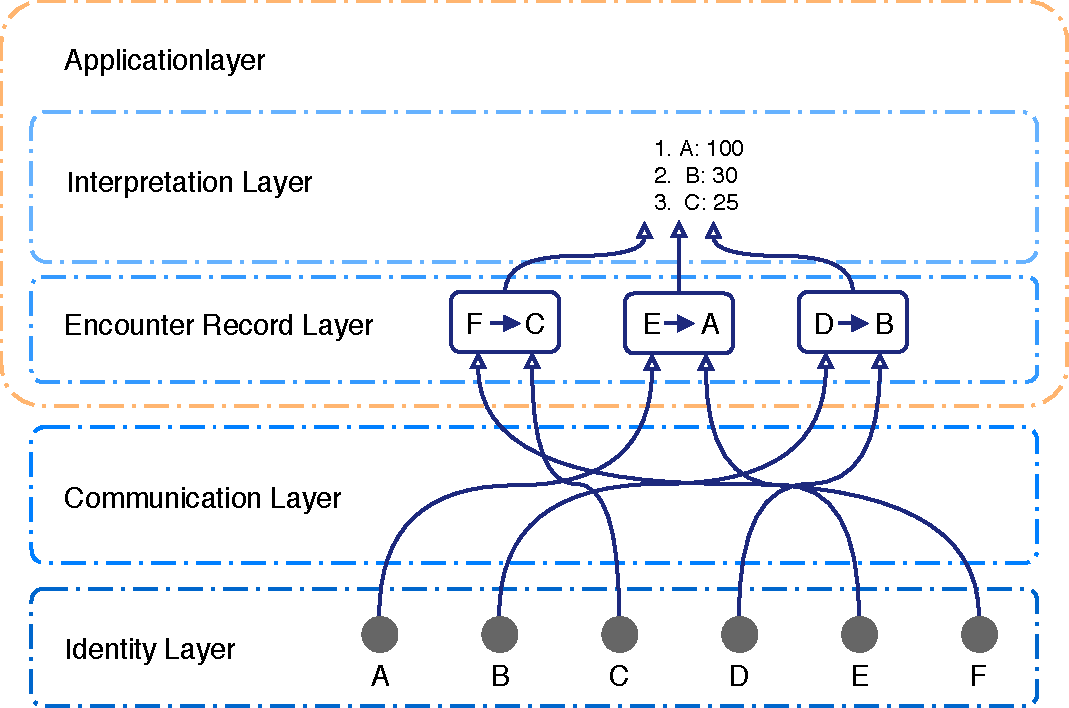
\includegraphics[width=\textwidth]{images/layers_of_trust_systems.pdf}
    \caption{Layered structure of our trust system architecture. The Identity Layer ensures the authenticity.
    The Communication Layer allows for point-to-point connections. The Encounter Record Layer ensures 
    the correctness of records. The Interpretation Layers allows to calculate reputation and trust of 
    peers. Both the encounters and their interpretation happen within a certain Application Context.}
    \label{fig:layers_of_trust_system}
\end{figure}

%     \item identity layer: digital identities are related to real-world entities and can either be real-people or entities like institutions or companies. The most simple first solution is just to identify entities by their public-private key pair.
%     * encounter record and distribution layer: encounters between digital identities needs to be recorded and distributed. Encounters are the basis for the reputation of entities, but reputation is only useful if it is gossiped such that other people can make decisions on the knowledge they have.
%     * interpretation layer: based on the known history of encounters, a reputation can be given to the known entities and decisions can be based on this. This layer contains the reputation function: NetFlow, MaxFlow, PageRank etc.

Each layer adds another level of protection: if identities are expensive and hard to create, fake 
identities will be less likely, protecting the system against spamming. Creating an immutable
record of each interaction and distributing that information to everyone makes agent's histories tamper-proof, unchangeable and reliable.
On the interpretation layer additional securities can be 
enabled: we envision a concept of locality to secure against distributed attacks with global 
collaborations of malicious nodes - if we only trust agents with a certain level of latency 
attackers can only choose from nodes in the vicinity and supply of those nodes is limited. 

Each of these components poses major challenges to the designers of a trust system. Yet we find 
that especially the recording, distribution and verification of encounters is crucial to the 
success of the trust system. Records of encounters are at the basis of the calculation of
reputation and trust. Thus, any open challenge in this layer will propagate up into the layer
of reputation, trust and the application context.

\section{Manipulation resistant interaction histories}
We now describe in more detail the challenges of ensuring the correctness of interaction records.

First, we should discuss the value of reputation and trust. In order to build a good reputation,
people act pro-socially at a personal cost which is rewarded with other people acting pro-socially 
towards them. Reputation is valuable because people with higher 
reputation can expect more cooperation in future interactions. This indirect reciprocity mechanism 
works as long as agents agree on what is good and what is bad reputation. Once there is ambiguity 
about the reputation of agents this value decreases. 

Agents base their perceived reputations of other agents on the knowledge about past interactions of 
their peers. In a centralized system all user's actions are observable by the single central entity. 
But this is generally not true for distributed systems as interactions are generally hard to to observe.
On the other hand, using only one's own history of interactions as indicator for our peers reputation
is also not an option. In a trust system with millions of users chances are high that users interact
with many previously unknown people. Instead agents need to acquire knowledge about their peers
transactions to make better decisions and reward those with a good reputation. This is possible with
epidemic gossiping: agents report new interactions to other agents who further spread those news. 
This is a natural process that also happens in the real-world trust building process~\cite{nowak2005evolution}.

Two main challenges of this process can be identified. Firstly, how can we ensure that agents are honest
about their own interactions? We have established that reputation has a value to agents. That could
lead to agents reporting a manipulated history which is better than the true history in order to 
obtain that value for free. Agents can protect against misreporting by exchanging information with 
each other and verifying that they ``heard the same'' about another or others. This leads to the 
second challenge: how can we ensure that agents take part in this process of exchanging and verifying
information? Although each honest agent benefits from banning dishonest agents from the network, an
agent can still argue to only report an agent that directly defrauded him. Checking any other 
behavior of the partner does not directly benefit him. It is therefore a social dilemma: if all 
agents help with verifying each other, everyone will benefit. Yet a single verifier has only little 
influence.

% Agreement on the interpretation layer can be achieved by defining a function for all agents to use
% which calculates a quantitative reputation from the history of feedback. Usually this history is 
% public, visible to everyone, however this is difficult to achieve in a distributed system. Here the
% second problem comes into play. The information a network node acts upon 
% is a different subset of complete information on the network for each agent; each agent is 
% in a different state. This situation is undesirable but inherent to systems with the requirements 
% stated in the previous section. Thus, a first step towards agreeing on the reputation of agents is 
% if agents agree on which data should be used as an input to the reputation function. In 
% other words we have to make sure that agents disseminate their knowledge and obtain knowledge from 
% other agents such that information is well distributed and available.

% However, in most contexts sharing and obtaining information comes at a cost which is not negligible.
% Thus agents may be reluctant to spend resources without any direct reward. There is an obvious 
% network effect to agents knowing more about their peers but agents can also gain reputation by 
% cooperating with agents with low reputation. Thus there is no incentive to obtain a better view of
% the network.

\section{Research question}
With the previous discussion about the challenges of reporting interactions, we can define a scope
for this work. We are aiming to facilitate honest reporting in a global trust system in order to 
create a basis for valid reputation and trust calculations. The challenge of this system is to 
ensure the integrity of these reports. 

Consequently, the question that we are trying to answer is therefore:
\begin{center}
    \textit{How to ensure that reports of encounters are honest, consistent and disseminated in a distributed trust system?}
\end{center}


% How to record, disseminate and protect the records of interactions in a global trust system?
% How to ensure honest reporting, distribution and verification of encounters in a global trust system?
% How to ensure that reports of encounters are honest, distributed and verified in a distributed trust system? 

In our research question we state three desireable properties of encounter reports that our system 
should enforce.

\begin{itemize}
    \item \textbf{Honest.} A record of an encounter
    includes an action performed by both agents. In the simplest case, as in the model we introduced to
    the reader in this chapter, this is simply cooperation or defection. The actions need to be honest 
    in order to rely on them for trust calculations. Similarly the order of encounters and the participating
    parties need to be honestly reported.
    \item \textbf{Consistent.}  We need to make 
    sure that only one version of each encounter can exist. Multiple versions of the same encounter
    leads to ambiguity of agents histories and thus invalid trust calculations.
    \item \textbf{Disseminated.} Reputation can only be valuable
    if it is spread through the network. Instead of spreading reputation directly, we require to 
    spread the knowledge of encounters such that each agent is able to determine their peers' reputation
    and whether to trust them or not.
\end{itemize}

Our reporting systems is supposed to be used as the basis for a global scale, distributed trust system. 
From this description we can extract specific requirements for the reporting system.

% 2. The reputation system we define needs to have some properties:

\begin{itemize}
    \item \textbf{Distributed.} No entity should be owner of the reputation of all people, no single point of
    failure should exist.
    \item \textbf{Scalable.} Future applications similar to those that exist today with centralized reputation
    systems should be able to handle billions of users.
    \item \textbf{Manipulation-resistant.} Once reputation increases in worth users of the 
    system will try to exploit it through attacks, alone or by colluding
\end{itemize}

Next to the properties defined in the research question, these practical requirements set boundaries
for the solution that we can propose.

\section{Related work}
\label{sec:related_work}
Before defining our own solution to the chosen problem we explore existing approaches.

\subsection{Replicated state machines}
The problem that we described in this section can be generalized to the problem of replicated 
state machines. The state of a reputation system depends on the interactions between agents. Each 
new encounter changes this state. The true state can be described by evaluating all records of 
encounters. Each agent in the trust system stores a subset of these records . Based on the records
agents are able to approximate the global system state. If all agents have the exact same records, 
they are able to agree on the state of the system. 

Replicated databases are a practical application in which this problem also arises. Early work from
Demers et al.\cite{demers1987epidemic} introduces the anti-entropy mechanism
for the purpose of maintaining mutual consistency between multiple replicas of a database. Updates
to the database can arrive at any single site and need to be forwarded to all other replicas. 
Anti-entropy is a process in which each database periodically 
chooses a random other instance and both exchange all database contents in order to resolve any 
differences between the two. In this work we will study a similar mechanism for exchanging records
of interactions between agents. 

Later similar processes of epidemic information spreading were summarized under the label of 
\textit{gossiping}. In distributed systems randomly chosen pairs of agents communicate to share 
knowledge. Both agents' knowledge base is combined and both agents will further spread the combined
information set in their following encounters. Note that this is a scientifically well-defined 
concept. different from the previously mentioned gossip in communities to facilitate indirect reciprocity.
We will subsequently refer to this well-defined concept when mentioning gossip \cite{hedetniemi1988survey}.

Very recent work combines the anti-entropy approach with a hashchain solution. Baird proposes a 
byzantine fault tolerant consensus scheme for replicated state machines~\cite{baird2016swirlds}. Similar
to the anti-entropy mechanism nodes in the network randomly connect and exchange all their knowledge. In each
such encounter new transactions can be announced. By signing each encounter and connecting it to the
previous encounters using their hashes, a hash graph is created which records the communication 
between all agents. Peers gossip about gossip and thus know what each of their peers have heard of and
know. A byzantine fault tolerant consensus mechanism is defined based on the hashgraph.

In this work we make use of two core concepts described in this section. Firstly, the anti-entropy
mechanism will be studied as an example for synchronizing the states of agents. This allows for 
agreement on reputations and trust, as well as fast dissemination of encounters with few necessary
connections. Also, we will define an architecture for recording those exchanges, similar to Hashgraph.
On the other hand, our architecture allows also for different exchange mechanisms that require less
bandwidth than anti-entropy. Also agents do not need to actively gossip when not interacting: instead
we propose to exchange information prior to any interaction.

\subsection{Blockchain systems with global consensus}
Replicated state machines were the predecessors of Bitcoin~\cite{nakamoto2008bitcoin} which created 
a whole new interest in distributed systems by releasing a concept and implementation for digital payments 
without banks. Bitcoin's innovation is mostly a combination of multiple existing concepts into a (new) technology, called blockchain.

Although the application context is a different one, the problem of recording transactions between
automated agents is very similar to our problem. Bitcoin was adopted quickly for anonymous digital 
payments. But its adoption layed bare scalability problems in the architecture. The proof-of-work
algorithm increases its complexity with more active nodes and keeps the transaction throughput 
constant. This leads to a theoretical bound of 60 transactions per second \cite{gervais2016security}. 
Other similar concepts were proposed with Litecoin~\footnote{https://litecoin.org}, Monero~\footnote{https://getmonero.org}
and Dashcoin~\footnote{http://dashcoin.info/} which add minor improvements over Bitcoin.
Ethereum~\cite{wood2014ethereum} was the first blockchain based fabric that allowed the decentralized
execution of scripts in addition to simple transactions. However it struggles with similar scalability
issues as Bitcoin.

In current development are proposals for increasing transaction throughput in blockchain-based 
systems, through so-called layer-2 solutions. One proposal introduces off-chain transactions in a protocol called the Lightning network~\cite{poon2016bitcoin}.
Two nodes deposit some Bitcoins into a channel. Afterwards they can use the channel for any number
of transactions. Once they agree to stop transacting, a net settlement is published. Only the 
opening and closing of channels leads to transactions on the blockchain, all transactions on the 
channel itself is only recorded locally. Multiple hops through channels are also possible such that 
if $A$ has a channel with $B$ and $B$ has a channel with $C$, a can perform a transaction with $C$. 
Although the lightning network improves scalability by allowing for an unlimited number of off-chain 
transactions, locking funds in each open channel can be problematic. Also, if channel creation and 
maintenance is expensive, a natural result is that certain nodes keep channels with many other 
nodes to act as an off-chain hub. This leads to centralization.

Another development is sharding. By splitting the network into several sub-networks, called shards.
Each shard records and secures its own state. As the network grows, new shards can be added, thus 
increasing the overall throughput of the system with increasing size. Although this seems like a 
good solution, problems arise when transaction need to be performed between shards. Elastico~\cite{luu2016secure}
uses a sharding solution with a Byzantine consensus scheme and allows for almost linear scalabilty.
However, inter-shard transactions are not possible.

Other innovations focus more on the consensus algorithm itself. Proof-of-work is not only slow but
also very energy-intensive \cite{bitcoin_energy}. Therefore other consensus protocols have been 
proposed and implemented such as Proof-of-State (POS) and Delegated-POS \cite{bentov2016cryptocurrencies, kiayias2017ouroboros}.
In the POS consensus mechanism, nodes do not need to expend computational resources to create a 
total sequence of blocks but rather bet some of their resources (stake) on a new block being the
next on the chain. Betting on the wrong block or a faulty block will lead to loss of those resources.
The stake to participate as a validator can be high, leading to centralization of power at the largest
stakeholders. Delegated-POS allows each node to vote on a set of validator. The decentralization is
re-established but by decreasing the parties involved in the validation of new blocks, the mechanism
is not as secure as Proof-of-Work.

\subsection{Pairwise accounting and pairwise ledgers}
In parallel to the blockchain development a different variation of replicated state machines was 
developed in the form of pairwise accounting systems. Instead of announcing transactions to all 
nodes in the network and ensuring global consensus, in pairwise accounting systems interactions are
initially only observed by the participating agents. Through employing some dissemination mechanims they are
broadcast to other agents. With respect to the previously introduced systems which enforce global 
consensus, this solution makes for a scalable, though less secure, transaction record. However, there is no 
guarantee on which information agents are acting and consistency cannot be ensured.

Meulpolder et al.\ propose BarterCast, a system that records transactions in the BitTorrent network
and selects future peers by their perceived reputation. The reputation is based on maxflow 
calculation of the interaction graph with agents being nodes and past transactions being edges. The
goal was to detect and ignore lazy free-riders who do not upload in the BitTorrent network \cite{meulpolder2009bartercast}.
In later work other mechanisms were proposed to be more resistant to dishonest reporting and sybil
attacks \cite{seuken2010accounting, seuken2014sybil}.

However the BarterCast system did not have any tamper-proof recording so the accounting mechanisms were
vulnerable to manipulations. Therefore, recent work by Otte et al.\ proposes a blockchain-based, pairwise
ledger which provides a tamper-evident scalable ledger. Transactions are 
entangled with two hash pointers to previous transactions. A transaction is confirmed by two parties
without requiring consensus with the rest of the network. We will describe this solution in detail 
in Chapter \ref{chap:implementation} because it will be the basis for the extension this work
introduces. 

Similar to TrustChain, IOTA is a distributed ledgers without global 
consensus~\cite{popov2016tangle}. Transactions are initially only recorded by the participating agents. A proof-of-work 
algorithm is used to work against spamming of transactions but not to obtain global consensus. Each
transactions is related to two other transactions that are confirmed. This creates a directed 
acyclic graph (DAG). A graph structure can grow much faster than a single global chain. DAG based 
ledgers therefore solve the largest problem of blockchain solutions: scalability.

Although DAG ledgers are superior to blockchain solution in terms of scalability, their weakness is
consistency. Nodes are not guaranteed to act on the same information about transactions. This can 
lead to conflicts about the validity of transactions. It is key to incentivize agents to acquire 
information from other agents and verify any new transaction against their knowledge. In this work
we propose a mechanism that guarantees this behavior.

\subsection{Reputation systems}
In our introduction we have mentioned the reputation systems of Airbnb and Uber as examples of 
state-of-the-art commercial systems for creating trust on the internet. Other such systems like 
eBay's reputation system for auctions have been more in the focus of research. It was found in 
multiple studies that a good reputation positively influences future interactions~\cite{resnick2002trust, houser2006reputation, dewan2004adverse}.

\cite{josang2007survey} is a very extensive survey of trust and reputation systems. The authors 
discuss among other things different definitions of trust and reputation, centralized and decentralized architectures 
of reputation systems as well as examples of commercial and live reputation systems. Apart from 
eBay, commercial reputation systems can be found in expert sites like AskMe\footnote{http://www.askmecorp.com},
sites that offer product reviews like Amazon\footnote{https://www.amazon.com}, discussion fora, 
for example Slashdot\footnote{https://slashdot.org}, Google's\footnote{https://google.com} page ranking which uses the PageRank
algorithm\cite{page1999pagerank} and Scientometrics. \cite{HENDRIKX2015184} is a more recent survey of reputation systems. They defined a 14 dimensional
taxonomy to compare reputation systems, among them governance which is either distributed or 
centralized. 

All commercial systems use a centralized
architecture. Centralized architectures record interaction feedback on servers who handle all 
communications with users. A central server can guarantee the security and integrity of records of
interactions as it a single source of truth. As discussed in Chapter \ref{chap:introduction} we do
not see a central solution as a viable option. 

\cite{HENDRIKX2015184} also mentions many academic reputation systems, a majority of those targets 
the decentralized governance scheme, mostly in peer-to-peer file sharing applications, such as EigenTrust~\cite{kamvar2003eigentrust},
PGrid~\cite{aberer2003p} and XRep~\cite{damiani2002xrep}.Although reputation system are much related to our use case, most work has been done on the 
the calculation of reputation rather than the secure storage of records. Also, they mostly have a
conceptual description of the reputation system rather than a software implementation that is proven
to work.

\subsection{Other work}
In \cite{haeberlen2007peerreview} the system PeerReview is proposed which records in a tamper-proof
hashchain the messages that each agent sends and receives. This allows each agent to verify that 
other agents act according to a reference implementation. In our work we use a similar approach but
optimize the system for the recording of two party transactions instead of a general messaging scheme.
This allows for a simpler witness selection process: each future transaction partner is a witness and
failing to perform the verification will also mark witnesses as a fraud.


% Transactions need to
% be verified by other agents and compiled into blocks. Publishing a correct block leads to a reward,
% yet a puzzle needs to be solved in order to do it. All nodes compete at solving the problem which 
% requires a lot of computing power. The puzzle difficulty increases wiht


% \begin{itemize}
%     \item Blockchain systems for recording transactions
%     \item Reputation systems, which ones talk about how to record and exchange information? Most of them probably concerned with calculation of trust
%     \item Distributed databases, how updates are disseminated
% \end{itemize}

% {\color{red}
% \begin{itemize}
%     \item First and second generation crypto currencies
%     \item Reputation systems
%     \item Dissemination mechanisms
%     \item Conclusion nothing does it all
% \end{itemize}}

% In the previous two chapters we have shown that a need exists for a decentralized accounting system 
% in order to create a global infrastructure for secure, anonymous digital transactions that does not 
% require control through a trusted third party. This need has been identified before and work has 
% been performed both in the scientific community as well as the industry. In this chapter we will 
% summarize those efforts, describe the short-comings of those approaches and define a basis for the 
% work performed in this work.

% \subsection{Dissemination mechanisms}
% Achieving the desired dissemination of transaction records is not a new problem in distributed 
% system as it is similar to synching the two stateful disconnected systems, for example a database.
% Dissemination mechanisms have been researched for many decades. \cite{hedetniemi1988survey} is an 
% early summary of the most important techniques in on dissemination Hedetniemi et al. describe 
% gossiping, broadcasting and shortly mention receiving and polling. We shall briefly introduce the 
% concepts here.

% \paragraph{Gossiping} Gossiping is the a mechanism in which pairwise exchange of information takes 
% place. Imagine a set of agents in which each agent has knowledge of a unique set of encounters that
% all other agents are not aware of. The goal is to reach a state in which all agent have the
% information on all encounters. During gossipping, an agent chooses a set of partners and with each 
% partner the agent exchanges all information. This is done by each agent and after a certain number
% of interactions the dissemination is complete. Different variants exist for gossiping, for example
% only allowing one-way communication, allowing multi-party exchanges and restricting the number of 
% exchanges per agent. 

% \paragraph{Broadcasting} Broadcasting is a process in which information originates from one 
% agent in the network, who needs to transmit the information to all other agents in the system. Again
% information transmission happens in pairs of two agents, and communication only happens between 
% adjacent nodes in the network. In contrast to gossiping where new information originates at all 
% nodes, in broadcasting all nodes communicate one piece of information.

% \paragraph{Receiving} In receiving all agents send some unique information to a specific agent, called
% the receiver. 

% \paragraph{Polling} Polling a information accumulation process in which a single originating agent sends requests for
% information to all other agents who then respond with an information carrying message. 

% The survey shows that dissemination of information in itself is a well understood topic and many 
% implementation of such protocols are widely available. However some problems exist when taking into
% account the possibility of strategic manipulation. Those will be discussed in the next section.


% \subsection{Decentralized accounting systems}
% The general concept of accounting is quite old as it is simply a recording of transactions between
% two or more parties. Before the digital age those recordings were simply written text on paper, 
% nowadays those recordings are stored in databases. We are concerned with another type, namely 
% decentralized accounting systems. We identified three types of applications for decentralized 
% accounting systems: cryptocurrencies, distributed work systems and reputation systems. 

% In the years 2007 and 2008 the global financial crisis shattered the global economy, lead to many
% people loosing house and job and diminished the trust clients had in banks to keep their money safe.
% Politics discussed the problem and proposed to regulate the banks more but with little impact. 
% However something else promised to change the banking world: the first white-paper for a 
% decentralized digital currency without any need for a trusted third party, Bitcoin, was announced. 

% \paragraph{Bitcoin.}
% Before the announcement of Bitcoin it was assumed that in order to verify the correctness of 
% transactions between parties and prevent cheating with digital money a bank or credit card company
% was needed. Bitcoin proved them wrong by creating a hash-based chain of transaction blocks, a global 
% ledger, that is shared among all users of the network. The acceptance of transactions is managed by 
% a process called ``mining'' which ensures that only the majority of CPU power can publish new 
% block. A blocks contains a fixed number of transactions and the Bitcoin network makes sure that a
% block is created once every 10 minutes. All mining node will execute the proof-of-work mechanism: 
% in order to publish a block a value needs to be found that, when hashed with a certain hashing 
% function like SHA-256, starts with a certain number of zeros. Depending on how many CPUs are active
% on the network the problem can be increased in difficulty by requiring more zeros at the beginning 
% of the hashed value. Once a new block is published other nodes will validate the transactions and 
% if they agree, will show their acceptance by working on creating the next block. This system ensures
% that as long as a majority of CPU power is owned by honest nodes, they will outpace the rest of the
% network in solving the hashing puzzle and creating valid blocks. Nodes will accept the longest chain
% and the transactions will be valid.

% The Bitcoin approach solved many problems assuming that an honest majority exists: first and 
% foremost the double-spending of funds is prevented because the Bitcoin blockchain creates one global
% order of valid transactions. Also the Sybil-attack is prevented by pairing the voting power to the
% available CPU power, which means Sybils can only run on real hardware, removing the advantage of
% fake identities. But these measures of attack prevention come at a price of efficiency. The surging 
% price of Bitcoins especially in the year 2017 led to a surge in transactions, transaction fees and
% energy usage. The increasing price of Bitcoins makes mining them more profitable which means more 
% nodes are joining the mining operation. Therefore the difficulty for the proof-of-work problem is 
% increased, such that it takes more computing power to find a correct value. This again increases the
% amount energy consumed in the whole network. At the same time the number of transactions processed
% is a constant of the Bitcoin currency, approximately 7 transactions per second. At the time of 
% writing the energy conusmption is at least 2.55 GW which makes it comparable to contries such as 
% Ireland. Summarized Bitcoin was a large step towards decentralized accounting but unsolved 
% scalability issues still prevent it from being actually useful as an infrastructure such as the one 
% we envision.

% \paragraph{Alternative coins and improvement measures.}
% Bitcoin served as a first proof-of-concept for trustless digital currencies or for our purposes, a
% ``secure'' decentralized accounting system, but the shortcomings were also obvious. Once the 
% populartiy increased, other enthousiasts, startups and incumbent companies started to create their 
% own spin-off digital currency. Each of these so-called ``alternative coins'' used blockchains as 
% a core technology to store transactions but tried to solve the scalability issues using different 
% approaches. The discussion of all alternative coins goes beyond the scope of this chapter, therefore
% we will quickly introduce some of the main differences between the largest systems. 

% The block time is one parameter to tweak in order to increase transaction throughput. Ethereum, the
% second largest cryptocurrencies currently uses a block time of 15 seconds with a proof-of-work 
% consensus. Also block size is a factor in the throughput rate, but increasing block time and size 
% only creates a constant factor to the rate of transactions.

% Ethereum is currently testing a proof-of-stake mechanism which should replace the energy intesive 
% proof-of-work. In short this mechanism will require ``minders'' to put some amount of currency into
% a wallet in order to participate in the process. If a miner does not perform the validation of 
% transactions correctly that ``stake'' will be lost for the miner. This will solve the energy 
% consumption problem but it will not solve the overall scalability issue of the system. 

% Another feature in development in multiple currencies is the ``Lightning network''. The lightning 
% network will allow two parties that expect to conduct multiple transactions with each other to 
% create a ``channel''. Both parties store some funds in the channel and can then interact freely 
% through this channel without needing to interact with the master network of the currency. Only the
% opening and netbalance at closing time will be writting to the chain while all other interactions 
% are only recorded locally. This should increase the possible throughput significantly but due to the
% early stages of development the actual implications of large-scale use are not proven at the time of
% writing. But considering that Bitcoin has a transaction limit of 200000 transactions a day, it would 
% still take 5000 days or 13.7 years to open one channel each for a billion people.

% The IOTA project ...

% Sharding ...

% Conclusion is no other system exists that fulfills the requirements


% \subsection{Distirubted work systems}
% In the field of distributed computing many applications include some mechanism in which a node is
% performing work for other nodes or the network in general. Seuken et al. call these distributed 
% work systems. Some examples of distributed work systems are peer-to-peer file-sharing network,
% packet forwarding in mobile ad-hoc networks and volunteer scientific distributed computing. As our 
% research group is mostly concerned with file-sharing networks and the concepts are similar in 
% general we will stick to that example to discuss the latest developments.

% Many different file-sharing networks have been built in the past, the most prominent being Napster,
% Gnutella and BitTorrent. In contrast to centralized file-sharing, in peer-to-peer systems there is 
% no server that contains all data, but instead users share data directly, one peer downloading and 
% one peer uploading. With no infrastructure needed, no costs and no single point of failure such a
% systems seems optimal. Talking in terms of distributed work systems, the act of uploading is 
% equivalent of performing work while the act of downloading consumes work. There is, however, a 
% social dilemma here: uploading to another node does not lead to an immediate reward for the
% uploading node, therefore, if we assume that bandwidth is a precious resource it is cheaper to not 
% upload, yet if all agents on the network realize this, no agent will upload and thus no agent is 
% able to download. The agents that do not upload any data are known as free-riders and free-rider 
% protection in peer-to-peer file-sharing networks is a subject of ongoing research.

% Accounting systems pose a possible solution to the free-riding problem. Let's first imagine a 
% centralized accounting systems keeping track of all uploading and downloading behavior, uploading 
% data increases the balance of agents, downloading decreases the balance. Now, the accounting system
% can enforce that agents keep their balance around 0, so they upload approximately as much as they
% download. Therefore, an accounting system can solve the free-riding problem, however as mentioned 
% multiple times, a decentralized accounting system is hard to implement. Accounting mechanisms have
% first been related with this subject in the DropEdge paper, however a lot of work has been done on
% the very related subject of reputation systems, which will be discussed in the next section. Seuken
% et al. define an incentive-compatible accounting mechanism which removes any advantage for users 
% that misreport their own contributions in the network. They present their DropEdge algorithm and 
% show that it's possible to increase the efficiency of BitTorrent clients using accounting. A 
% negative result of their work is that an accounting mechanism cannot prevent sybil attacks. Some
% short-comings of the approach is strategic manipulations of data and dissemination of data. 

% \subsection{Reputation systems}
% One of the reasons that decentralized accounting systems are hard to create is that agents in
% peer-to-peer applications do not have a complete view of the network and thus also not all 
% information of the network, at least not without a global consensus mechanism. In the file-sharing
% example from the previous section agents decide to upload to other agents based on some partial 
% knowledge of the network and contributions of agents. It can be argued that an accounting mechanism
% cannot be correct if it acts on partial information and instead the particular balance of an agent 
% as seen by another agent is rather a reputation. The goal is then to create trust between users in 
% order to facilitate cooperation. Such a system will be called a reputation system. 

% Whether reputation systems can be called an application of accounting systems can be argued about. 
% In general accounting systems track transactions between accounts, the full history of transactions
% determines the state of the network. According the framework of Mui et al. trust is the expectation
% of reciprocation for an agent given that agent's history of behavior. So a reputation system can act 
% on the data of an accounting system and add additional conclusions. The previous example of agents
% uploading and downloading helps to understand this. An accounting system keeps track of the 
% transactions and calculates the balance of an agent, for example +10MB, for an agent that has 
% uploaded 10MB more than downloaded. Also it is possible to account the total uploaded and downloaded
% data, for example 1010MB and 1000MB respectively. A simple accounting system stops at this point, 
% the system behaves correctly when no error has been done in calculating the balances and the data is
% correct. A reputation system adds another layer of interpretation to this data. The simplest 
% reputation function only checks whether the balance is positive or not, or if the choice is between
% multiple agents, whose balance is the most positive. Another reputation function might weight agents
% with a 0 balance but 10GB of uploaded (and downloaded) data more trustworthy than an agent with 10MB
% positive balance but only 100MB uploaded data. Thus we can see a reputation system as a layer on top
% of an accounting system.

% Describe some reputation systems ...
% \section{Agent behavior through incentive}

% \section{Scope}